\chapter{Introduction to Set Theory}
\markright{Chapter \ref{ch:introsettheory}: Set Theory}
\label{ch:introsettheory}
\setlength{\parindent}{1em}

\section{What is a set?}

One of the major advantages that predicate logic has over propositional logic is that it enables us to \emph{quantify} over a collection of objects. Because propositional logic is only about complete sentences in a language, we don't have the ability there to talk about how some objects are related to other objects, or to talk about all the objects there are.

However, predicate logic still has some limitations. It is unwieldy in predicate logic to talk about \emph{specific} quantities. Consider the following first order sentence:
\[\exists x \forall y (Fx \eand (Fy \rightarrow x=y))\]
This sentence says that there is an object, x, that has property $F$ and that for any other object y, y has $F$ only if x and y are identical. This sentence is equivalent to the English sentence ``There is only one F.''

We can extend this approach to create greater and greater quantities, if we want. We can even say things like ``There are between three and seven Fs that are also Gs.'' However, these sentences get unwieldy extremely fast.

To help us talk about collections of objects in a more precise and concise way, we are going to introduce some new logical machinery. We are going to introduce the notion of a set.

\newglossaryentry{set}
{
name=Set,
description={A set is an abstract collection of objects that are unique and unordered.}
}

A \textsc{\gls{set}} is an abstract. mathematical object that represents a collection of objects. There are a few restrictions on sets that we'll discuss in a bit. First, let's just look at the notation for sets.

We notate sets with capital letters like $X$, $Y$, or $Z$. Some authors will also put sets in boldface, but we won't do that here. The contents of a set can be represented in one of two ways. The first way to represent the contents of a set is \emph{extensionally}, which means we simply list all the objects in the set one by one:
\begin{figure}
\[X=\{a,b,d,e,1,2,3\}\]
	\caption{A set defined extensionally.}
	\label{fig:setextension}
\end{figure}
We can put anything we like into a set, but each object is only listed once. We call the objects inside of a set the \textsc{\glspl{element}} of that set. We also always surround the elements of a set with curly braces to indicate that they are together inside of the set.

The other way to define a set is \emph{intensionally} which means we give an unambiguous condition that tells us whether or not an object is in the set. Suppose we want to create a set that contains all and only the even natural numbers. Such a set would be defined intensionally as follows:
\begin{figure}
\[\mathbb{E}=\{n \in \mathbb{N} | n \text{ is even.}\}\]
	\caption{A set defined intensionally.}
	\label{fig:setintension}
\end{figure}
We read this as ``The set of even integers is equal to the set that contains all natural numbers such that the natural number is even.'' That's pretty wordy, but the basic idea is straightforward. Unlike in an extensional definition where we simply list the elements of the set inside the curly braces, an intensional definition has two parts. On the lefthand side is the ``population'' or the collection of all the objects that \emph{could} be in the set. On the righthand side is the ``condition'' which an element from the population must satisfy in order to be in our set. So in the example above, we are drawing from the set of all the natural numbers and only putting the even ones into our new set.

What kinds of things can go in a set? Anything you like! You can construct sets of numbers, letters, colors, dogs, cats, clouds, planets, or anything else! However, there are some restrictions on the objects that go in a set. The first restriction is \emph{uniqueness}. This means that for any set only \emph{one} of each object can be in the set. Let's see an example.

Suppose we want to create a set of all the animals at the zoo. We start off listing the animals as follows: \[Z=\{penguin, tiger, elephant, koala, elephant, giraffe, lion, turtle\}\]. Notice that we've listed `elephant' twice! This is not permitted when constructing sets so we have to remove the duplicate: \[Z=\{penguin, tiger, elephant, koala, giraffe, lion, turtle\}\].

When we want to say whether or not something is an element in a set, we use the symbol $\in$. This symbol is called the ``set membership'' symbol. Used in a sentence, the symbol looks like this: $tiger\in Z$. That sentence is true, but the sentence $zebra\in Z$ is false. To say that something is \emph{not} in a set we can add a negation symbol out front, as in $\enot(zebra\in Z)$, or abbreviate this sentence by writing a slash through the set membership symbol: $zebra\not\in Z$.

Our set $Z$ tells us all of the \emph{kinds} of animals at the zoo, but what if we want a set that contains each individual animal? We can do that, but we need some way of showing that animals of the same species are distinct. We can do this in a number of different ways, but the preferred way is to give the animals a \emph{unique} name or identifier:

\[Z`=\{penguin_1, penguin_2,\ldots, elephant_1, elephant_2, \ldots,koala_1, koala_2, koala_3, \ldots\}\]

We could just as easily give them unique names like Bob and Sue, but this way we preserve some information about their species.

We can also put sets inside of other sets! Consider the following set:

\[Z*=\{\{penguin_1, penguin_2,\ldots\}, \{elephant_1, elephant_2, \ldots\},\{koala_1, koala_2, koala_3, \ldots\}\ldots\}\]

Now we have a set that contains more sets---one for each exhibit in our zoo.

There's no limit to how many nested sets there can be! We can nest sets indefinitely if we want to, just like Matryoshka dolls.\begin{marginfigure}
	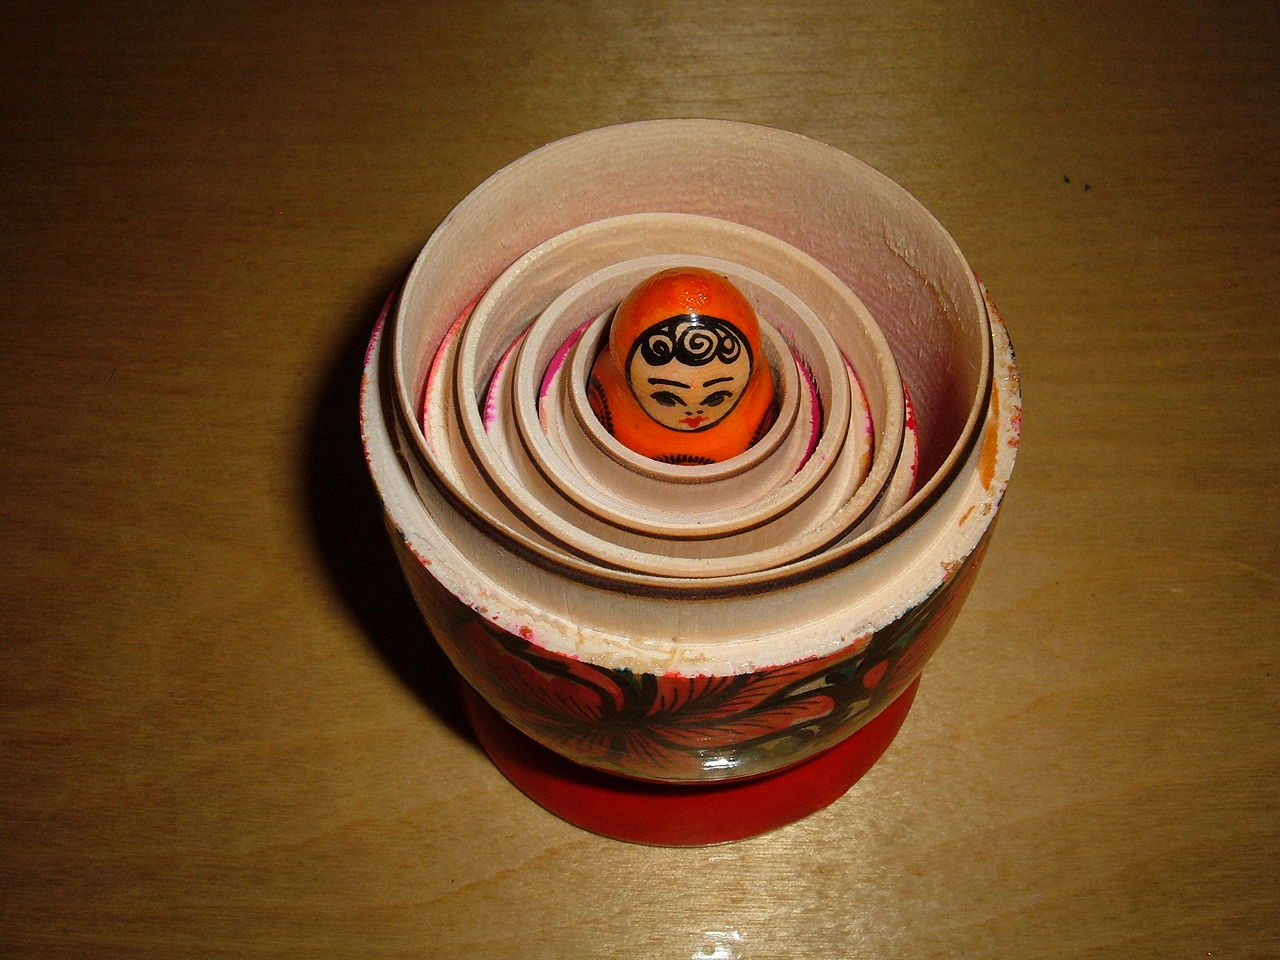
\includegraphics[width=\textwidth]{matryoshkadoll}
	\caption{A Russian nesting doll.}
	\label{fig:matryoshkadoll}
\end{marginfigure}

\section{Counting Sets}

We call the number of elements in a set the \textsc{\gls{cardinality}} of the set. We represent the cardinality of a set with vertical bars like this:
\[\text{If }A=\{cat, dog, sandwich\}\text{, then }|A|=3\]
It's important to remember that the cardinality of a set is just a property of that set. Different sets can have the same cardinality, but that doesn't mean that they are the same set. Sets are identified by their members, not by their size.


We can also have a set with no members
